Today I'm only attending one session and a keynote.

\subsection{Session: Game Theory and Fairness}

As with the other sessions, there will be one longer talk (20min) followed by 5 minute spotlights.

\subsubsection{Optimizing Generalized Rate Metrics with Three Players \cite{narasimhan2019optimizing}}

Talk by Harikrishna Narasimhan. \\

Focus: solve constrained learning problems!. So:
\[
\min_\theta P(\theta)\ s.,t. P^j(\theta) \leq \eps, \forall_{j \in \mathbb{N}}.
\]
Example: fair hiring. We want to ensure that we minimize our F-measure, while ensuring equal precision (to be unbiased in hiring). \\

{\bf Main Q:} How does one design learning algorithms to handle general performance metrics and constraints? \\

Problem setup:
\[
\min_\theta \psi(R_1(\theta), \ldots, R_k(\theta)),
\]
such that:
\[
\psi^j(R_1(\theta), \ldots) \leq 0,\ j =1, 2, \ldots
\]

Where there are K prediction rates:
\[
R_k(\theta) = \bE_{(X,Y)}[I(Y \neq \tx{sign}(f(X)))].
\]

Prior methods:
\begin{enumerate}
    \item Solution A: use surrogates!
    \begin{itemize}
        \item Relax indicators with continuous surrogates
        \item Relaxing constraints with surrogates may make the problem infeasible
        \item Surrogates may output values outside the range of $\psi$
    \end{itemize}
    \item Solution B: Cost-weighted minimization oracle (breaks problem into simpler sub problems)
\end{enumerate}

{\bf This Paper:} General framework which recovers prior methods as special cases. Also use to develop practical algorithms with minimal use of surrogate and tight handling. \\

Heart of framework:
\begin{itemize}
    \item Min-Max game formulation:
    \[
    \min_{\theta} \psi^j(R_1(\theta), \ldots) \ldots
    \]
    \item Replace these functions with slack variables to decouple rates:
    \[
    \min_{\theta, \chi} \psi(\chi_1, \ldots)
    \]
    \item Then induce a Lagrangian min-max problem
\end{itemize}

Three player viewpoint: 1) $\lambda$-player, linear, 2) $\chi$-player, convex, 3) $\theta$-player:
\[
\min_{\theta, \chi}\max_{\lambda \geq 0} \psi(\ldots) - \sum_k \lambda_k \chi_k + \sum_k \lambda_k R_k(\theta)
\]
Then, surrogate based algorithm:
\begin{enumerate}
    \item $\chi$-player: best response
    \item $\lambda$-player: SGD with indicators
    \item $\theta$-player: SGD with surrogates: only works with last objective ($R_k(\theta)$).
\end{enumerate}

Prove: near-optimal approach for original learning problem, and near-feasible for constraints. Also prove results related to finding mixed nash and coarse correlated equilibrium. \\

Big advantage: new algorithms with guarantees, can also handle non-convex functions of prediction rates. \\

Experiment: try to maximuze the F-measure subject to a constraint on the F-measure of a minority. \\

Open source library: \durl{https://github.com/google-research/tensorflow_constrained_optimization}.


\subsubsection{Modeling Conceptual Understanding in Image Reference Games}

Talk by Rodolfo Corona. \\

{\bf New game:} image-reference game played by pairs of agents, where the listener sometimes can't distinguish aspects of the image. So:
\begin{itemize}
    \item Speaker (agent 1) must described image to listener
    \item Description must be a single attribute
    \item But, sometimes the listener can't perceive aspects of the object (colorblind, for instance) 
    
    $\ra$ Speaker then plays sequences of games with listeners that can't perceive attributes of objects and must {\it learn} to adapt to different listeners.
\end{itemize}

Experiments: take a meta-learning approach! Explore in practice games to get to know the listener, before having to adapt. \\

$\ra$ Compare against a random practice game baseline, speaking baseline in contrast. Meta-learning exploration approach works quit well.\\

$\ra$ Performed ablation study and found that it was {\it crucial} that the speaker explicitly model aspects of the listener. \\

Strong performance in adapting to new speakers on the CalTech birds dataset (real images!). 

\subsubsection{This Looks Like That: Deep Learning for Interpretable Image Recognition \cite{chen2019looks}}

Talk by Oscar Li. \\

Q: Look at a bird! What kind of bird is it? More generally: how do we answer this question? \\

A: We tend to look for specific features that are indicative of a class. \\

{\bf Proposal:} Draw inspiration from how people identify classes to form a new kind of interpretability with richer explanations. \\

$\ra$ New model ProtoPNet: provides a new kind of interpretability with highlighting in an image, but also adds an explanation as to why those pieces where chosen. \\

Training algorithm:
\begin{enumerate}
    \item SGD of layers before last layer
    \item Projection of prototypes
    \item Convex optimization of last layer.
\end{enumerate}

Experiments: Achieve near state of the art performance on benchmark dataset, and carry out analysis of latent space.

\subsubsection{Assessing Social and Intersectional Biases in Word Representations \cite{tan2019assessing}}

Two main Questions: 1) Do embedding association tests demonstrate social bias on contextual word encodings in the test sentence? 2) Can we develop comprehensive test for gender, race, and intersectional identities? \\

$\ra$ Focus on {\it contextual} word encoding, since they tend to improve downstream NLP performance, and do not have the problem of obfuscation. \\

Example Q: How related is concept X with attribute A, and concept Y, with attribute B? As opposed to X with B, and Y with A? (example concepts: names, attributes: stereotypically male/female occupation). \\

Study two concepts: gender, race, and a bunch of relevant attributes like occupation, likability, and so on. \\

$\ra$ Main contribution: new approach for finding intersectional biases in embeddings.


\subsubsection{Paradoxes in Fair Machine Learning \cite{golz2019paradoxes}}

Talk by Anson Kahng. \\

Q: What is the relationship between fairness in machine learning and fairness in fair division? \\

Fairness in ML: statistical notions of fairness.

Fairness in FD: axioms of fair division (resource monotinicity). \\

{\bf Setting:} classification with cardinality constraints. So, a classification problem with a fixed budget of available resource to distribute, e.g. financial aid. \\

$\ra$ Find a classifier that maximizes efficiency. But, two views on fairness: classification and fair division.\\

Fair Division Axioms: resource monotonicity (can't make people worse off with more resources), population monotonicity (if someone leaves the pool, it can't hurt).\\ 

$\ra$ The axioms are roughly in place to preclude paradoxes.

New Q, then: How much does efficiency suffer if we must satisfy these axioms, too? \\

\ddef{Equalized Odds}{A predictor $\hat{Y}$ satisfies equal odds w.r.t protected attribute on Y if $\hat{Y}$ and $A$ are independent conditional on $Y$}

Results:
\begin{enumerate}
    \item In the cardinality constrained model, we characterize optimal allocation rule that satisfies equalized odds.
    \item Equalized odds and resource monotonicity are achievable with no loss to optimal equalized odds efficiency.
    \item Any rule that satisfies equalized odds and population monotonicity can't achieve a constant factor approximation to optimal equalized odds efficiency.
\end{enumerate}

\spacerule


\subsection{Keynote: Jeffrey Heer on Agency and Automation}

Some of us are weery about the current rhetoric about AI, in part due to hype, but also because it is so focused on {\it pure autonomy}, rather than a harmonious combination of people with machines. \\

%{\it ``I worry that enthusiasm for AI is prevent us from reckonig with its looming effects on society, if we want it to play a positive role in toorows world it must be guided by human concerns, not replacing us." -- Fei-Fei Li}

20 years ago: work by Eric Horvitz on ``Principles of Mixed-Initiative User Interfaces". Studies: 1) support uncertainty around user goals, 2) allow efficient direct invocation and termination, and 3) continue to learn by observing user actions. \\

$\ra$ lots of work since then, too! \\

60 years ago: Bar-Hillel said {\it ``Fully automatic high quality translation is not a reasonable goal, not even for scientific texts. A human translator in order to arrive at high quality output, is often obliged to make intelligent use of extra-linguistic knowledge which sometimes has to be of considerable breadth and depth."} \\

{\bf Long standing design challenge:} determine regions of optimality in possible divisions of labor among directed and autonomous actions. \\

Fundamental Q: what is the appropriate balance between automation and user control? \\

Many challenges;
\begin{itemize}
    \item Automated mehtods may be biased or inaccurate
    \item Consequences of poor models let loose in the world
    \item Loss of critical engagement and domain expertise
    \item Ambiguity of human intent, cognitive biases, mistakes
    \item Often lack a global view.
\end{itemize}

{\bf Proposed Strategy:} Shared representations that enhance user interfaces with models of capabilities, actions, and goals to reason about principled human-AI collaboration. \\

Three examples:
\begin{enumerate}
    \item Data cleaning and data visualization.
    \item Data cleaning and transformation.
    \item Natural language translation
\end{enumerate}

\subsubsection{Data Cleaning and Data Visualization}

Let's think about {\it topic models} like Latent Dirichilet Allocation (LDA). We don't just care about the output, we would prefer this have some relevant structure such as text-order and other relationships---these can help us digest, search through, and process the findings of the topic model. \\

$\ra$ One thing learned: users of these data/systems are quite savvy! Running the same LDA leads to different results, perhaps contrast the results of different models to gain further insight into the right kinds of representations. \\

Recent work: mapping machine-learned latent spaces into something visualizable that people can understand. This can let us {\it align} the learned latent space to something we can make sense of. \\

{\bf Broad Question:} What makes a visualization {\it good}? \\

$\ra$ A quick experiment: how much bigger is the small shape than the larger shape?
\begin{itemize}
    \item Two circles, one big one large, asked to guess the precise relative size of the two.
    
    $\ra$ Really high variance in audience responses!
    
    \item Same task but with two bar charts.
    
    $\ra$ Really low variance in responses.
\end{itemize}

But: the two ratios were identical, but people were much more concentrated around the right answer in the latter case. \\

$\ra$ Can turn to psychophysics to rank visual encodings quantitatively; people are good at determining position, length, slope, but not as effective with color, volume, and area. \\

{\bf Common Exploration Pitfalls:} 1) Overlook data quality issues, 2) Fixating on specific relationships, 3) Plus many other biases. \\

\begin{figure}[h!]
    \centering
    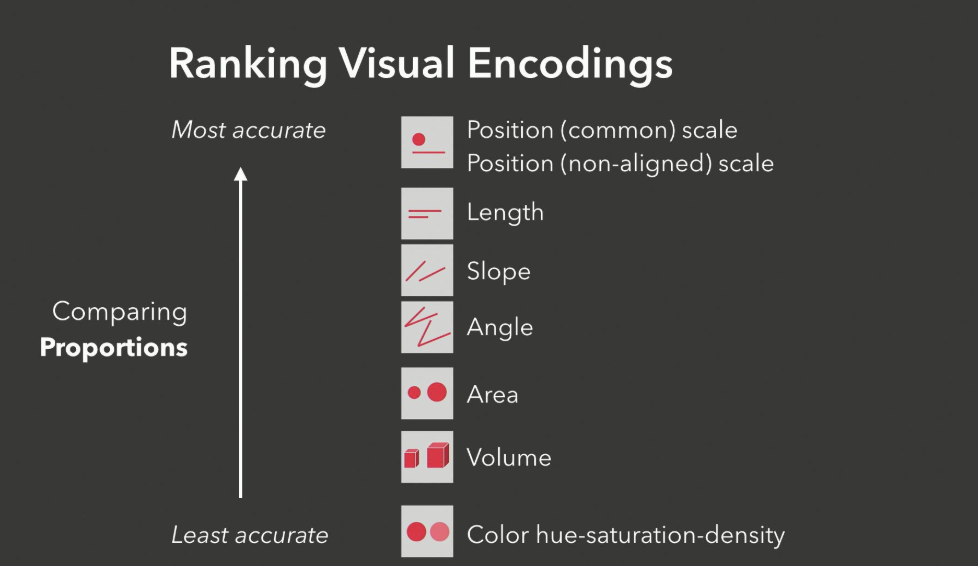
\includegraphics[width=0.7\textwidth]{figures/psychphys.png}
    \caption{Different accuracy for people in estimating quantities of visual stimuli}
    \label{fig:psychphys}
\end{figure}

{\bf Project:} Visual exploratory tool for large datasets, use inference in the background to automatically recommend new visuals. Can also be taught how to create these plots by the tool itself. \\

{\bf Key Idea from Demo:}
\begin{enumerate}
    \item Augment manual exploration with visualization recommendations sensitive to the user's current focus. 
    \item Ultimate goal is to support systematic consideration of the data without exacerbating false discovery.
    \item To model a user's search frontier, we optimize for related chart specifications, seeded current focus.
\end{enumerate} 
    

Representative quotes about the tool:
\begin{itemize}
\item Related view suggestion accelerates exploration a lot
\item I like that it show what fields to include to see a specific graph
\item The related views are so good but it's spoiling that I start thinking less. I'm not sure if that's a good thing
\end{itemize}

\subsubsection{Data Cleaning and Transformation}

Quote from Anonymous Data Scientist: {\it ``I spend more than half my time integrating, cleansing, and transforming data without doing any actual analysis. Most of the time I'm lucky if I get to do any 'analysis' at all"}

$\ra$ Responses; that can't be true! I wish I only spent 50\% of time on data cleaning.. (see big data borat on twitter).\\

{\bf New System:} DataWrangler (2011). DataWrangler: tool for generating relational datasets based on input preferences of user! Taught the system to automate aspects of the data cleaning process, but also generates a {\it program} that does the data cleaning. We can extract this program and use it for other thing, too.\\

$\ra$ ``Predictive Interaction": has an underlying domain specific language that can be used to ``lift" the program to generate visualizations and interactions. These lifted components can be used to inform a {\it guide-decide} loop for end users. \\

Also ran user studies with this system:
\begin{itemize}
\item Reduces spec time, promotes use of reusable scalable transformations.

\item Complementarity: suggestions good for tasks people found hard (extraction patterns, etc). People good in cases where inference is less tractable
\item Agency: Users appreciated suggestions in respond to an initiating interaction, but did not always act on practice assistance.
\end{itemize}

$\ra$ Company called Trifacta uses this interaction system and the discovered paradigms to scale the software to production. \\


\subsubsection{Natural Language Translation}

Started the talk with 1960s quote from Bar-Hillel---around this time there was a clear vision for interactive translation and interfaces. Even a proposal for an interactive translation workflow. \\



% \begin{figure}[h!]
%     \centering
%     \includegraphics[width=0.7\textwidth]
%     caption{Proposal for early interactive translation interface}
%     \label{fig:my_label}
% \end{figure}

$\ra$ Two big challenges, though: 1) Translation wasn't {\it good} enough to be a reliable collaborator, and 2) Getting these interface designs right is also challenges. \\

But! Revisited recently: predictive translation memory (PTM).

Again conducted user studies for interactive machine translation.
\begin{itemize}
\item Experiments with professional translators across language pairs (Arabic, French, German to English) and text genres (software, medical, news)
\item Results: 
\begin{itemize}
    \item Post-editing of full translation leads to reduced time and improved quality (over manual translation)
    \item Interactive translation with PTM slightly slower than post-editing but yields higher quality translations
    \item {\bf Similar concerns around agency:} ``I feel less susceptible to be creative", and ``distracts from my own original translation process by putting words in my head."
\end{itemize}


\end{itemize}


{\bf Design Challenge:} Determine regions of optimality in possible divisions of labor among directions and autonomous agents. \\

Future Challenges:
\begin{enumerate}
    \item {\it Design process, tools, and monitoring:} how might we support productive prototyping, development,  deployment, using machine learning?
    
    \item {\it Mapping machine-learned representations:} Can ML methods suggest structural task models? can people help test an constrain ML models?

    \item {\it Evaluating Trade-Offs of Agency and Automation:} Must go beyond results of quality and productivity.
    
    $\ra$ Locus of control, agency vs passive acceptance? Training and skill acquisition vs. de-skilled labor?
\end{enumerate} 

